% Created by tikzDevice version 0.12.3.1 on 2022-09-02 14:22:31
% !TEX encoding = UTF-8 Unicode
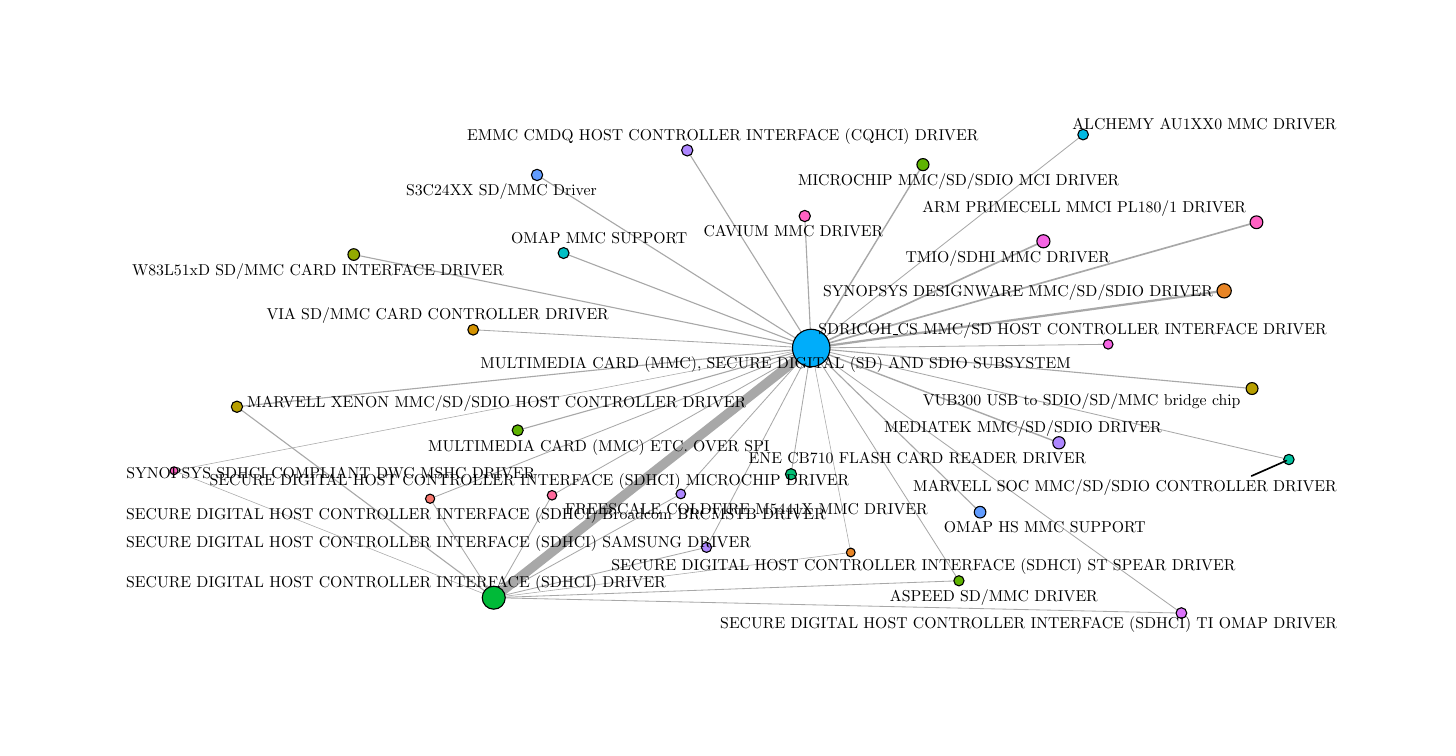
\begin{tikzpicture}[x=1pt,y=1pt]
\definecolor{fillColor}{RGB}{255,255,255}
\path[use as bounding box,fill=fillColor,fill opacity=0.00] (0,0) rectangle (505.89,252.94);
\begin{scope}
\path[clip] (  0.00,  0.00) rectangle (505.89,252.94);
\definecolor{fillColor}{RGB}{255,255,255}

\path[fill=fillColor] (  0.00,  0.00) rectangle (505.89,252.94);
\end{scope}
\begin{scope}
\path[clip] ( 32.75, 32.75) rectangle (475.89,222.94);
\definecolor{drawColor}{gray}{0.66}

\path[draw=drawColor,line width= 0.3pt,line join=round] (381.38,214.30) -- (283.13,137.18);

\path[draw=drawColor,line width= 0.6pt,line join=round] (444.02,182.62) -- (283.13,137.18);

\path[draw=drawColor,line width= 0.3pt,line join=round] (336.51, 53.07) -- (283.13,137.18);

\path[draw=drawColor,line width= 0.3pt,line join=round] (336.51, 53.07) -- (168.41, 46.96);

\path[draw=drawColor,line width= 0.4pt,line join=round] (280.79,184.88) -- (283.13,137.18);

\path[draw=drawColor,line width= 0.4pt,line join=round] (238.33,208.61) -- (283.13,137.18);

\path[draw=drawColor,line width= 0.3pt,line join=round] (275.83, 91.58) -- (283.13,137.18);

\path[draw=drawColor,line width= 0.3pt,line join=round] (236.01, 84.45) -- (283.13,137.18);

\path[draw=drawColor,line width= 0.3pt,line join=round] (236.01, 84.45) -- (168.41, 46.96);

\path[draw=drawColor,line width= 0.3pt,line join=round] (455.75, 96.89) -- (283.13,137.18);

\path[draw=drawColor,line width= 0.4pt,line join=round] ( 75.62,115.96) -- (283.13,137.18);

\path[draw=drawColor,line width= 0.4pt,line join=round] ( 75.62,115.96) -- (168.41, 46.96);

\path[draw=drawColor,line width= 0.5pt,line join=round] (372.64,102.93) -- (283.13,137.18);

\path[draw=drawColor,line width= 0.5pt,line join=round] (323.51,203.45) -- (283.13,137.18);

\path[draw=drawColor,line width= 0.4pt,line join=round] (177.07,107.44) -- (283.13,137.18);

\path[draw=drawColor,line width= 0.4pt,line join=round] (283.13,137.18) -- (344.15, 77.86);

\path[draw=drawColor,line width= 0.4pt,line join=round] (283.13,137.18) -- (193.65,171.50);

\path[draw=drawColor,line width= 0.4pt,line join=round] (283.13,137.18) -- (184.06,199.72);

\path[draw=drawColor,line width= 0.3pt,line join=round] (283.13,137.18) -- (390.44,138.53);

\path[draw=drawColor,line width= 0.3pt,line join=round] (283.13,137.18) -- (145.41, 82.72);

\path[draw=drawColor,line width= 3.4pt,line join=round] (283.13,137.18) -- (168.41, 46.96);

\path[draw=drawColor,line width= 0.3pt,line join=round] (283.13,137.18) -- (189.47, 83.97);

\path[draw=drawColor,line width= 0.3pt,line join=round] (283.13,137.18) -- (245.30, 65.14);

\path[draw=drawColor,line width= 0.2pt,line join=round] (283.13,137.18) -- (297.42, 63.30);

\path[draw=drawColor,line width= 0.3pt,line join=round] (283.13,137.18) -- (416.89, 41.40);

\path[draw=drawColor,line width= 0.8pt,line join=round] (283.13,137.18) -- (432.35,157.85);

\path[draw=drawColor,line width= 0.2pt,line join=round] (283.13,137.18) -- ( 52.89, 92.84);

\path[draw=drawColor,line width= 0.6pt,line join=round] (283.13,137.18) -- (367.03,175.75);

\path[draw=drawColor,line width= 0.3pt,line join=round] (283.13,137.18) -- (160.98,143.78);

\path[draw=drawColor,line width= 0.4pt,line join=round] (283.13,137.18) -- (442.43,122.54);

\path[draw=drawColor,line width= 0.4pt,line join=round] (283.13,137.18) -- (117.82,170.96);

\path[draw=drawColor,line width= 0.3pt,line join=round] (145.41, 82.72) -- (168.41, 46.96);

\path[draw=drawColor,line width= 0.3pt,line join=round] (168.41, 46.96) -- (189.47, 83.97);

\path[draw=drawColor,line width= 0.3pt,line join=round] (168.41, 46.96) -- (245.30, 65.14);

\path[draw=drawColor,line width= 0.2pt,line join=round] (168.41, 46.96) -- (297.42, 63.30);

\path[draw=drawColor,line width= 0.3pt,line join=round] (168.41, 46.96) -- (416.89, 41.40);

\path[draw=drawColor,line width= 0.2pt,line join=round] (168.41, 46.96) -- ( 52.89, 92.84);
\definecolor{drawColor}{RGB}{0,0,0}
\definecolor{fillColor}{RGB}{0,185,227}

\path[draw=drawColor,line width= 0.4pt,line join=round,line cap=round,fill=fillColor] (381.38,214.30) circle (  1.92);
\definecolor{fillColor}{RGB}{255,97,195}

\path[draw=drawColor,line width= 0.4pt,line join=round,line cap=round,fill=fillColor] (444.02,182.62) circle (  2.31);
\definecolor{fillColor}{RGB}{94,179,0}

\path[draw=drawColor,line width= 0.4pt,line join=round,line cap=round,fill=fillColor] (336.51, 53.07) circle (  1.84);
\definecolor{fillColor}{RGB}{255,97,195}

\path[draw=drawColor,line width= 0.4pt,line join=round,line cap=round,fill=fillColor] (280.79,184.88) circle (  2.04);
\definecolor{fillColor}{RGB}{174,135,255}

\path[draw=drawColor,line width= 0.4pt,line join=round,line cap=round,fill=fillColor] (238.33,208.61) circle (  2.04);
\definecolor{fillColor}{RGB}{0,191,116}

\path[draw=drawColor,line width= 0.4pt,line join=round,line cap=round,fill=fillColor] (275.83, 91.58) circle (  2.02);
\definecolor{fillColor}{RGB}{174,135,255}

\path[draw=drawColor,line width= 0.4pt,line join=round,line cap=round,fill=fillColor] (236.01, 84.45) circle (  1.74);
\definecolor{fillColor}{RGB}{0,193,159}

\path[draw=drawColor,line width= 0.4pt,line join=round,line cap=round,fill=fillColor] (455.75, 96.89) circle (  1.88);
\definecolor{fillColor}{RGB}{183,159,0}

\path[draw=drawColor,line width= 0.4pt,line join=round,line cap=round,fill=fillColor] ( 75.62,115.96) circle (  2.05);
\definecolor{fillColor}{RGB}{174,135,255}

\path[draw=drawColor,line width= 0.4pt,line join=round,line cap=round,fill=fillColor] (372.64,102.93) circle (  2.22);
\definecolor{fillColor}{RGB}{94,179,0}

\path[draw=drawColor,line width= 0.4pt,line join=round,line cap=round,fill=fillColor] (323.51,203.45) circle (  2.18);

\path[draw=drawColor,line width= 0.4pt,line join=round,line cap=round,fill=fillColor] (177.07,107.44) circle (  2.00);
\definecolor{fillColor}{RGB}{0,173,250}

\path[draw=drawColor,line width= 0.4pt,line join=round,line cap=round,fill=fillColor] (283.13,137.18) circle (  6.78);
\definecolor{fillColor}{RGB}{97,156,255}

\path[draw=drawColor,line width= 0.4pt,line join=round,line cap=round,fill=fillColor] (344.15, 77.86) circle (  2.10);
\definecolor{fillColor}{RGB}{0,191,196}

\path[draw=drawColor,line width= 0.4pt,line join=round,line cap=round,fill=fillColor] (193.65,171.50) circle (  1.98);
\definecolor{fillColor}{RGB}{97,156,255}

\path[draw=drawColor,line width= 0.4pt,line join=round,line cap=round,fill=fillColor] (184.06,199.72) circle (  2.05);
\definecolor{fillColor}{RGB}{245,100,227}

\path[draw=drawColor,line width= 0.4pt,line join=round,line cap=round,fill=fillColor] (390.44,138.53) circle (  1.74);
\definecolor{fillColor}{RGB}{248,118,109}

\path[draw=drawColor,line width= 0.4pt,line join=round,line cap=round,fill=fillColor] (145.41, 82.72) circle (  1.66);
\definecolor{fillColor}{RGB}{0,186,56}

\path[draw=drawColor,line width= 0.4pt,line join=round,line cap=round,fill=fillColor] (168.41, 46.96) circle (  4.16);
\definecolor{fillColor}{RGB}{255,105,156}

\path[draw=drawColor,line width= 0.4pt,line join=round,line cap=round,fill=fillColor] (189.47, 83.97) circle (  1.72);
\definecolor{fillColor}{RGB}{174,135,255}

\path[draw=drawColor,line width= 0.4pt,line join=round,line cap=round,fill=fillColor] (245.30, 65.14) circle (  1.82);
\definecolor{fillColor}{RGB}{232,133,38}

\path[draw=drawColor,line width= 0.4pt,line join=round,line cap=round,fill=fillColor] (297.42, 63.30) circle (  1.58);
\definecolor{fillColor}{RGB}{219,114,251}

\path[draw=drawColor,line width= 0.4pt,line join=round,line cap=round,fill=fillColor] (416.89, 41.40) circle (  1.94);
\definecolor{fillColor}{RGB}{232,133,38}

\path[draw=drawColor,line width= 0.4pt,line join=round,line cap=round,fill=fillColor] (432.35,157.85) circle (  2.58);
\definecolor{fillColor}{RGB}{255,97,195}

\path[draw=drawColor,line width= 0.4pt,line join=round,line cap=round,fill=fillColor] ( 52.89, 92.84) circle (  1.43);
\definecolor{fillColor}{RGB}{245,100,227}

\path[draw=drawColor,line width= 0.4pt,line join=round,line cap=round,fill=fillColor] (367.03,175.75) circle (  2.37);
\definecolor{fillColor}{RGB}{211,146,0}

\path[draw=drawColor,line width= 0.4pt,line join=round,line cap=round,fill=fillColor] (160.98,143.78) circle (  1.94);
\definecolor{fillColor}{RGB}{183,159,0}

\path[draw=drawColor,line width= 0.4pt,line join=round,line cap=round,fill=fillColor] (442.43,122.54) circle (  2.15);
\definecolor{fillColor}{RGB}{147,170,0}

\path[draw=drawColor,line width= 0.4pt,line join=round,line cap=round,fill=fillColor] (117.82,170.96) circle (  2.10);

\path[draw=drawColor,line width= 0.6pt,line join=round,line cap=round] (442.23, 90.93) -- (454.86, 96.50);

\node[text=drawColor,anchor=base,inner sep=0pt, outer sep=0pt, scale=  0.57] at (425.23,216.01) {ALCHEMY AU1XX0 MMC DRIVER};

\node[text=drawColor,anchor=base,inner sep=0pt, outer sep=0pt, scale=  0.57] at (381.77,186.00) {ARM PRIMECELL MMCI PL180/1 DRIVER};

\node[text=drawColor,anchor=base,inner sep=0pt, outer sep=0pt, scale=  0.57] at (349.15, 45.69) {ASPEED SD/MMC DRIVER};

\node[text=drawColor,anchor=base,inner sep=0pt, outer sep=0pt, scale=  0.57] at (276.69,177.37) {CAVIUM MMC DRIVER};

\node[text=drawColor,anchor=base,inner sep=0pt, outer sep=0pt, scale=  0.57] at (251.19,212.16) {EMMC CMDQ HOST CONTROLLER INTERFACE (CQHCI) DRIVER};

\node[text=drawColor,anchor=base,inner sep=0pt, outer sep=0pt, scale=  0.57] at (321.52, 95.45) {ENE CB710 FLASH CARD READER DRIVER};

\node[text=drawColor,anchor=base,inner sep=0pt, outer sep=0pt, scale=  0.57] at (259.71, 76.96) {FREESCALE COLDFIRE M5441X MMC DRIVER};

\node[text=drawColor,anchor=base,inner sep=0pt, outer sep=0pt, scale=  0.57] at (396.50, 85.51) {MARVELL SOC MMC/SD/SDIO CONTROLLER DRIVER};

\node[text=drawColor,anchor=base,inner sep=0pt, outer sep=0pt, scale=  0.57] at (169.46,115.66) {MARVELL XENON MMC/SD/SDIO HOST CONTROLLER DRIVER};

\node[text=drawColor,anchor=base,inner sep=0pt, outer sep=0pt, scale=  0.57] at (359.62,106.50) {MEDIATEK MMC/SD/SDIO DRIVER};

\node[text=drawColor,anchor=base,inner sep=0pt, outer sep=0pt, scale=  0.57] at (336.42,195.94) {MICROCHIP MMC/SD/SDIO MCI DRIVER};

\node[text=drawColor,anchor=base,inner sep=0pt, outer sep=0pt, scale=  0.57] at (206.42, 99.96) {MULTIMEDIA CARD (MMC) ETC. OVER SPI};

\node[text=drawColor,anchor=base,inner sep=0pt, outer sep=0pt, scale=  0.57] at (270.27,129.69) {MULTIMEDIA CARD (MMC), SECURE DIGITAL (SD) AND SDIO SUBSYSTEM};

\node[text=drawColor,anchor=base,inner sep=0pt, outer sep=0pt, scale=  0.57] at (367.54, 70.37) {OMAP HS MMC SUPPORT};

\node[text=drawColor,anchor=base,inner sep=0pt, outer sep=0pt, scale=  0.57] at (206.55,175.07) {OMAP MMC SUPPORT};

\node[text=drawColor,anchor=base,inner sep=0pt, outer sep=0pt, scale=  0.57] at (171.18,192.23) {S3C24XX SD/MMC Driver};

\node[text=drawColor,anchor=base,inner sep=0pt, outer sep=0pt, scale=  0.57] at (377.55,142.08) {SDRICOH{\_{}}CS MMC/SD HOST CONTROLLER INTERFACE DRIVER};

\node[text=drawColor,anchor=base,inner sep=0pt, outer sep=0pt, scale=  0.57] at (161.95, 75.21) {SECURE DIGITAL HOST CONTROLLER INTERFACE (SDHCI) Broadcom BRCMSTB DRIVER};

\node[text=drawColor,anchor=base,inner sep=0pt, outer sep=0pt, scale=  0.57] at (133.10, 50.52) {SECURE DIGITAL HOST CONTROLLER INTERFACE (SDHCI) DRIVER};

\node[text=drawColor,anchor=base,inner sep=0pt, outer sep=0pt, scale=  0.57] at (181.35, 87.55) {SECURE DIGITAL HOST CONTROLLER INTERFACE (SDHCI) MICROCHIP DRIVER};

\node[text=drawColor,anchor=base,inner sep=0pt, outer sep=0pt, scale=  0.57] at (148.45, 65.23) {SECURE DIGITAL HOST CONTROLLER INTERFACE (SDHCI) SAMSUNG DRIVER};

\node[text=drawColor,anchor=base,inner sep=0pt, outer sep=0pt, scale=  0.57] at (323.66, 56.64) {SECURE DIGITAL HOST CONTROLLER INTERFACE (SDHCI) ST SPEAR DRIVER};

\node[text=drawColor,anchor=base,inner sep=0pt, outer sep=0pt, scale=  0.57] at (361.67, 35.76) {SECURE DIGITAL HOST CONTROLLER INTERFACE (SDHCI) TI OMAP DRIVER};

\node[text=drawColor,anchor=base,inner sep=0pt, outer sep=0pt, scale=  0.57] at (357.87,155.90) {SYNOPSYS DESIGNWARE MMC/SD/SDIO DRIVER};

\node[text=drawColor,anchor=base,inner sep=0pt, outer sep=0pt, scale=  0.57] at (109.53, 90.02) {SYNOPSYS SDHCI COMPLIANT DWC MSHC DRIVER};

\node[text=drawColor,anchor=base,inner sep=0pt, outer sep=0pt, scale=  0.57] at (354.16,168.26) {TMIO/SDHI MMC DRIVER};

\node[text=drawColor,anchor=base,inner sep=0pt, outer sep=0pt, scale=  0.57] at (148.18,147.33) {VIA SD/MMC CARD CONTROLLER DRIVER};

\node[text=drawColor,anchor=base,inner sep=0pt, outer sep=0pt, scale=  0.57] at (380.85,116.46) {VUB300 USB to SDIO/SD/MMC bridge chip};

\node[text=drawColor,anchor=base,inner sep=0pt, outer sep=0pt, scale=  0.57] at (104.91,163.45) {W83L51xD SD/MMC CARD INTERFACE DRIVER};
\end{scope}
\end{tikzpicture}
